% !TeX document-id = {1c0b4298-276a-4038-8e08-c4a1f4846da7}
% !TeX TXS-program:bibliography = txs:///biber
\documentclass[10pt,a4paper]{article}
\usepackage[T1]{fontenc}
\usepackage{graphicx}
\usepackage{mathtools}
\usepackage{amssymb}
\usepackage{amsthm}
\usepackage{thmtools}
\usepackage{xcolor}
\usepackage{nameref}
\usepackage{hyperref}
\usepackage{color}
\usepackage{float}

\usepackage[
backend=biber,
style=authoryear,
natbib=true
]{biblatex}
\addbibresource{../bibliography.bib}


\title{\large EAE1223: Econometria III}
\author{\normalsize Exercícios de revisão para a P1}
\date{}
\begin{document}
	\maketitle
\begin{enumerate}
	
	\item[1] Dada uma série de tempo $Y_t$ com 230 observações, considere a estimação da seguinte especificação
	\begin{equation}
		\Delta Y_t = \alpha + \gamma \cdot Y_{t-1} + \sum_{s=1}^k \beta_k \cdot \Delta Y_{t-s} + u_t
	\end{equation}
	Na tabela abaixo, reportamos três quantidades: (1) o p-valor de $H_0: \gamma = 0$ contra $H_1: \gamma < 0$ baseado na estatística $\hat{t}$ e nos valores críticos tabulados por Dickey e Fuller; (2) a estatística $F$ do teste da nula conjunta $(\alpha, \gamma) = (0,0)$; (3) o p-valor de $H_0: \gamma = 0$ contra $H_1: \gamma < 0$ baseado na estatística $\hat{t}$ e em valores críticos normais.
	
	
	\begin{table}[H]
		\begin{center}
			\begin{tabular}{c|c}
				
				$p_{t,DF}$&0.8998    \\
				\hline
				$\hat{F}$&1.0292    \\
				\hline
				$p_{t,\text{Normal}}$&0.5606\\
			\end{tabular}
		\end{center}
	\end{table}
	No que segue, indique as conclusões do procedimento sequencial visto em aula, para um nível de significância de 10\%.
	\begin{enumerate}
		\item[(A)] Concluímos que a série \textbf{não} apresenta raiz unitária.
		\item[(B)] Concluímos que a série \textbf{apresenta} raiz unitária.
		\item[(C)] Concluímos que o modelo \textbf{não apresenta intercepto}. Nesse caso, devemos proceder à estimação do modelo sem intercepto, e realizar o teste $t$ baseado em valores críticos tabulados por Dickey e Fuller nesse modelo.
		\item[(D)] Nenhuma das alternativas anteriores.
	\end{enumerate}
	
	\item[2] Observando a FAC e FACP, assinale qual processo é mais provável de ter gerado os dados:
	
	\begin{figure}[H]
		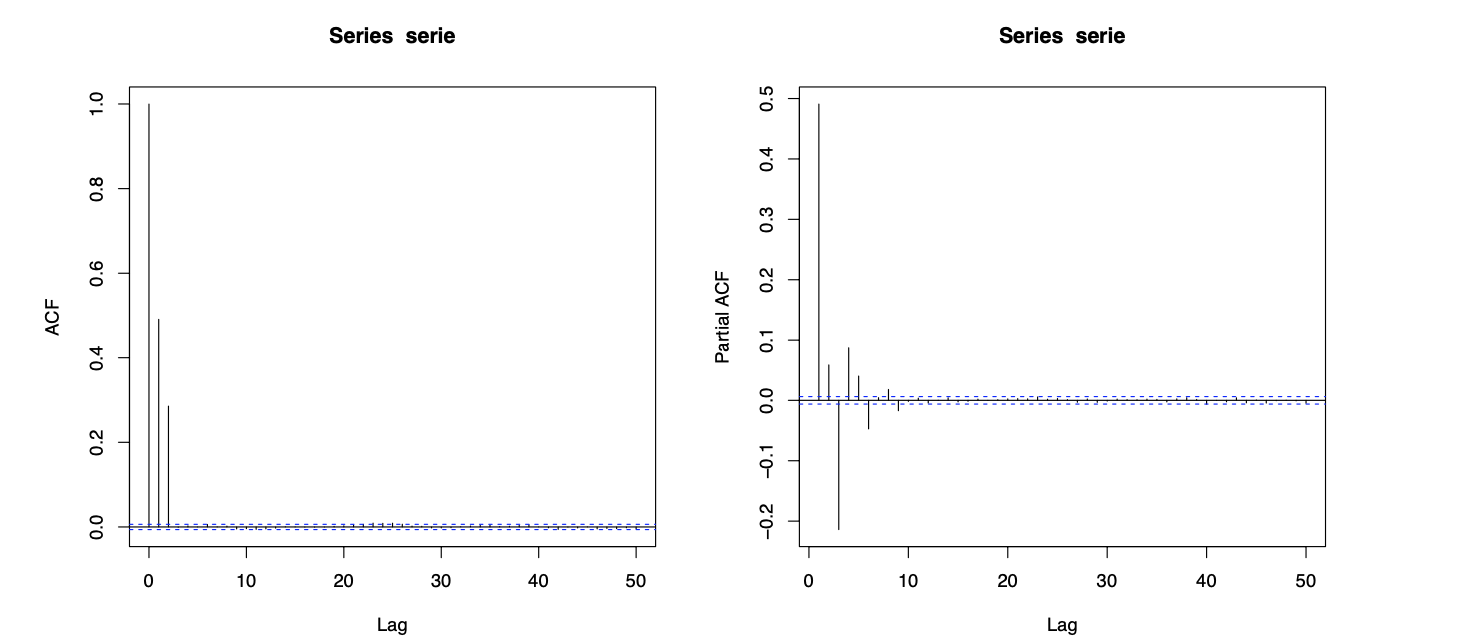
\includegraphics[scale=0.5]{figuras/fac_facp.png}

	\end{figure}
	
	\begin{enumerate}
		\item[(A)] ARMA(5,1)
		\item[(B)] AR(3) 
		\item[(C)] MA(3)
		\item[(D)] MA(2)
	\end{enumerate}
	
	\item[3] Considere o seguinte MA(1) Gaussiano.
	$$y_t = \epsilon_t + \theta_1 \epsilon_{t-1}\, ,$$
	onde $\epsilon_t \overset{\text{iid}}{\sim} N(0,\sigma^2)$.
	
	\begin{itemize}
		\item[a] Mostre que, para todo $t> 0$:
		
		$$y_t = \epsilon_t + \theta_1\left(\sum_{j=1}^{t-1}(-\theta_1)^{t-1 - j}Y_{j}  +  (-\theta_1)^{t-1}\epsilon_0\right)$$
		\item[b] Infira, do resultado acima, que:
		$$y_t|\epsilon_0,y_{1},\ldots, y_{t-1}\sim N\left(\theta_1\left(\sum_{j=1}^{t-1}(-\theta_1)^{t-1 - j}Y_{j}  +  (-\theta_1)^{t-1}\epsilon_0\right),\sigma^2 \right)\,.$$
		\item[c] Usando o resultado acima e que, para todo $t$ e $k <t$, a densidade conjunta de $(y_{k+1},\ldots, y_t)$ condicional a $(\epsilon_0,y_1,\ldots, y_k)$, $f_{y_{k+1},\ldots, y_t|\epsilon_0,y_{1,\ldots, y_k}}$, satisfaz:
		
		\begin{equation*}
			\begin{aligned}
						\footnotesize f_{y_{k+1},\ldots, y_t|\epsilon_0,y_1,\ldots, y_k}(y_{k+1},\ldots, y_t|\epsilon_0,y_1,\ldots, y_k)= \\ f_{y_{k+1}|\epsilon_0,y_1,\ldots, y_k}(y_{k+1}|\epsilon_0,y_1,\ldots, y_k) f_{y_{k+2},\ldots, y_t|\epsilon_0,y_1,\ldots, y_{k+1}}(y_{k+2},\ldots, y_t|\epsilon_0,y_1,\ldots, y_{k+1})
			\end{aligned}
		\end{equation*}
		Mostre que a densidade de $y_{1},\ldots y_{T}$, condicional a $\epsilon_0 = \tilde{\epsilon}_0$, satisfaz:
		
		$$f_{y_1,\ldots, y_T|\epsilon_0}(y_1,\ldots,y_T|\tilde{\epsilon}_0)=\prod_{t=1}^T \frac{1}{\sigma}\phi\left(\frac{y_t - \theta_1\left(\sum_{j=1}^{t-1}(-\theta_1)^{t-1 - j}Y_{j}  +  (-\theta_1)^{t-1}\tilde{\epsilon}_0\right)}{\sigma}\right)\, ,$$
	onde $\phi$ é a densidade de uma normal padrão, $\phi(x) = \frac{1}{\sqrt{2\pi}}\exp(-x^2/2)$.
	
	\item Mostre que o estimador $\hat{\theta}^{\text{MLE}}_1$ que maximiza a log-verossimilhança condicional:
	
	$$(\hat\sigma^{\text{MLE}}, \hat\theta_1^{\text{MLE}}) \in \operatorname{argmax}_{s> 0, c \in \mathbb{R}} \log\left(\prod_{t=1}^T\frac{1}{s}\phi\left(\frac{y_t - c\left(\sum_{j=1}^{t-1}(-c)^{t-1 - j}Y_{j}  +  (-c)^{t-1}\tilde{\epsilon}_0\right)}{s}\right)\right)$$
	\end{itemize}
	
	É \textbf{idêntico} ao estimador condicional de mínimos quadrados não lineares visto em aula.
\end{enumerate}
	
\end{document}